\documentclass[11pt,a4paper]{article}
\usepackage[utf8]{inputenc}
\usepackage[T1]{fontenc}
\usepackage[italian]{babel}
\usepackage{lmodern,geometry,graphicx,booktabs,amsmath,xcolor,hyperref,caption}
\geometry{margin=2.1cm}
\hypersetup{colorlinks=true,linkcolor=blue,urlcolor=blue}
\title{Confronto del solutore OOFEM con la letteratura\\\large Allen--Cahn parabolica e iperbolica}
\author{Report di validazione numerica}
\date{26 ottobre 2026}
\begin{document}
\maketitle
\begin{abstract}
Questo report raccoglie i confronti già eseguiti per rendere visibile cosa è stato verificato e con quale forza. Il risultato parabolico più concreto è il confronto 1D (striscia 2D uniforme) con l'energia pubblicata da Okumura. Inoltre, il test 2D con coefficienti unitari realizza il modello polinomiale di Calatroni--Colli: i raffinamenti numerici sono coerenti con il loro risultato teorico di esistenza e unicità, pur senza una soluzione chiusa da sovrapporre. Il test 2D con Xiao--Chen resta esplorativo, perché il paper non specifica il parametro di interfaccia. Per l'iperbolico, la replica dell'onda viaggiante di Nizovtseva et al. concorda con la soluzione esatta e mostra ordine spaziale vicino a due. Il profilo esatto di Hochbruck--Leibold è stato verificato con la forzante ricalcolata per l'operatore OOFEM, ma tale prova non riproduce l'equazione né il metodo del loro articolo; gli errori spaziali restano elevati.
\end{abstract}

\section*{Come leggere i risultati}
\textcolor{green!45!black}{\textbf{Confronto diretto}} significa che modello, dati e parametri del riferimento sono identificati e messi a confronto con risultati OOFEM. \textcolor{orange!80!black}{\textbf{Esplorativo}} indica che una discrepanza di dati o risoluzione impedisce una conclusione quantitativa. Le verifiche di convergenza con soluzioni esatte o indipendenti dimostrano proprietà del solver, ma non sono di per sé confronto con dati pubblicati.

\section{Ramo parabolico}
\subsection{Benchmark 1D di Okumura}
Il test riproduce il Computation Example 2, capitolo 4, della tesi di M. Okumura (2021): Allen--Cahn 1D con capacità dinamica agli estremi, $L=1$, $K=100$, capacità agli estremi $10$, coefficiente del potenziale $100$, dato iniziale $u_0(x)=\exp[-500(x-0.5)^2]$, $\Delta t=10^{-3}$ e orizzonte $T=0.7$. In OOFEM il problema 1D è rappresentato da una striscia Q1 con una fila uniforme in profondità; i contributi dinamici sono applicati ai due lati corti.

La figura confronta l'energia totale ricostruita da OOFEM con i punti digitalizzati dalla Fig. 4.4 della tesi. Sul tratto $0.01\le t\le0.4$, RMSE $=0.988$, MAE $=0.880$ e massimo scarto $=1.832$, mentre l'asse energetico del grafico copre circa 0--90. La curva OOFEM decresce monotonicamente. Il confronto è quantitativo ma la curva di riferimento è digitalizzata da un'immagine raster, perciò la lettura dei punti introduce incertezza. La forma del campo evolve coerentemente con la Fig. 4.3.

\begin{figure}[h!]
\centering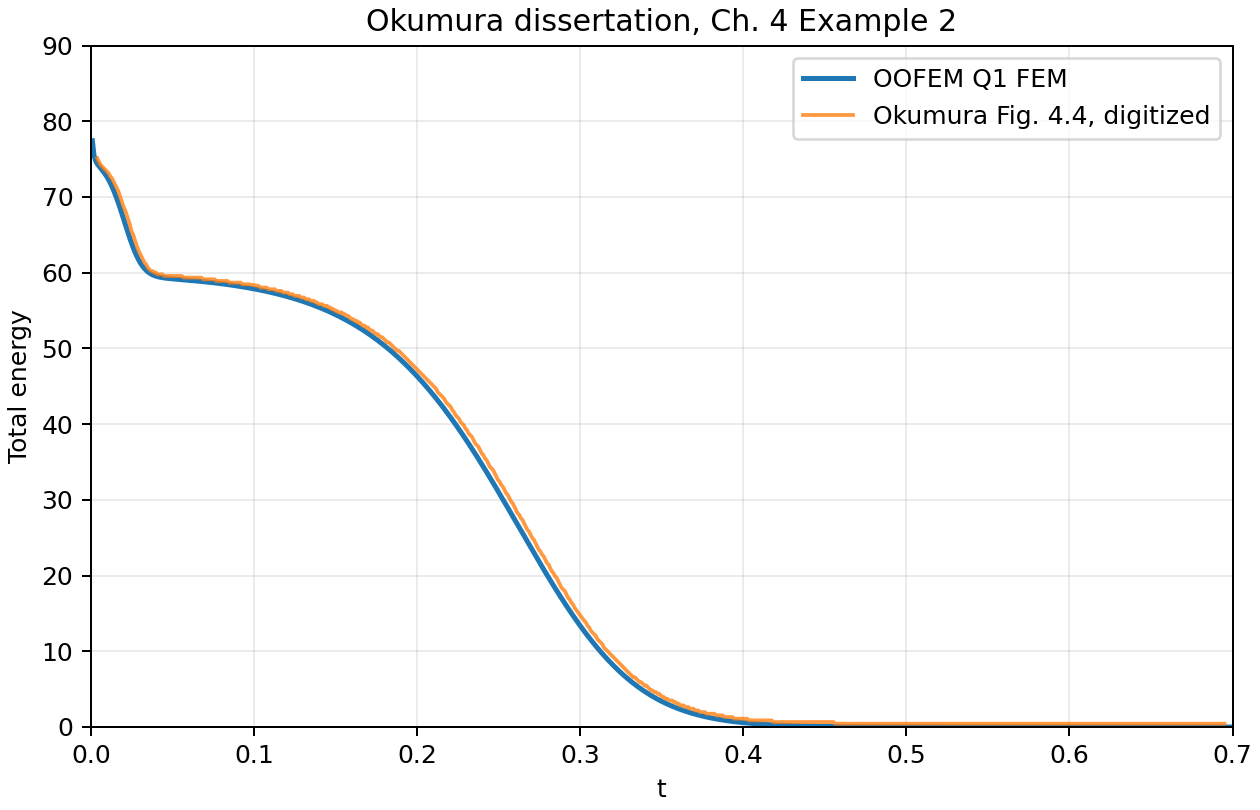
\includegraphics[width=.9\textwidth]{literature_comparison/okumura_ch4_example2_energy_overlay.png}
\caption{Energia OOFEM sovrapposta alla curva digitalizzata dalla letteratura. Questo è il confronto parabolico quantitativo principale.}
\end{figure}

\subsection{Test 2D di Xiao--Chen}
È stato eseguito il caso della goccia quadrata senza penalizzazione, su $20\times20$ quadrilateri, assumendo $\varepsilon=0.1$ e $\Delta t=10^{-4}$. A $T=0.1$ la posizione approssimata del contorno $u=0.5$ concorda visivamente con la figura pubblicata. L'ipotesi $\varepsilon=0.1$ non è però indicata nel paper per quel caso; inoltre la mesh OOFEM è molto più grossolana di quella dell'articolo e mostra sensibilità spaziale. Non confrontiamo energie assolute né dichiariamo validazione quantitativa 2D.

\begin{figure}[h!]
\centering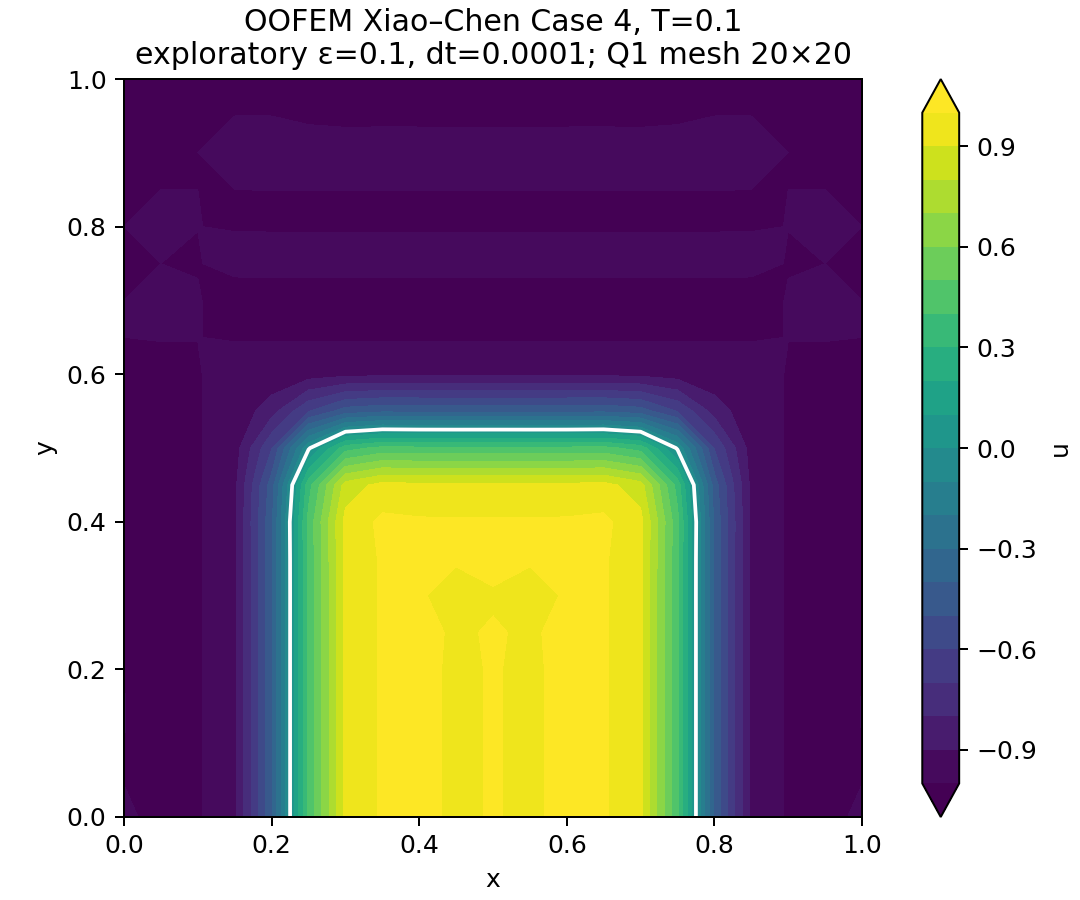
\includegraphics[width=.77\textwidth]{literature_comparison/xiao_chen_case4_exploratory_n20_dt0.0001.png}
\caption{Risultato esplorativo OOFEM 2D. L'immagine illustra la morfologia, non una replica parametrica completa del riferimento.}
\end{figure}

\subsection*{Verdetto parabolico}
Il caso 1D è supportato da un confronto diretto con dati naturali di letteratura, inclusi i parametri e il dato iniziale: la curva energetica concorda strettamente, tenendo conto della digitalizzazione. Il comportamento 2D del bordo con variazione tangenziale non è ancora validato quantitativamente contro il paper citato.

\section{Ramo iperbolico}
\subsection{Che equazione è effettivamente implementata?}
Nel solver corrente l'inerzia $u_{tt}$ è nel bulk; la frontiera conserva una legge Allen--Cahn dinamica del primo ordine nel tempo. È quindi un modello misto bulk inerziale / superficie dissipativa. I preprint CRC 1173/2018-53, 2019-26 e 2020-20 trattano invece onde/acustica con inerzia e termini cinetici al bordo (con varianti e smorzamenti propri). La sovrapposizione di argomento non basta per equiparare le equazioni: quei lavori sono riferimenti metodologici, non benchmark diretti del sistema OOFEM accoppiato.

\subsection{Controlli quantitativi del bulk}
Newmark medio è stato confrontato con (i) la soluzione esatta del sistema Q1 semidiscreto lineare per un modo coseno e (ii) un'integrazione indipendente DOP853 dell'oscillatore $u_{tt}=u-u^3$. Dimezzando $\Delta t$ da $0.04$ a $0.02$, l'errore RMS cala rispettivamente di fattore circa 4 e l'ordine osservato è 2.00 e 2.02.
\begin{figure}[h!]
\centering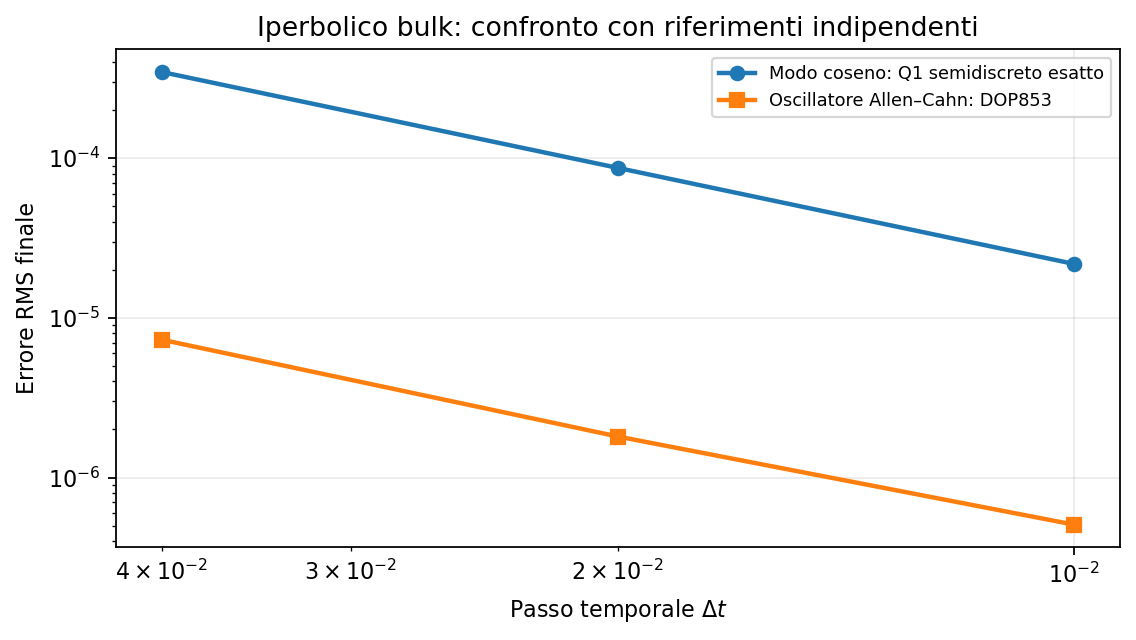
\includegraphics[width=.82\textwidth]{comparison_report_figures/hyperbolic_time.png}
\caption{Errore finale dei test bulk rispetto ai riferimenti indipendenti. La pendenza vicina a due è coerente con Newmark medio.}
\end{figure}

\subsection{Profilo kink e sistema accoppiato}
Il profilo stazionario $\tanh(x/\sqrt2)$, soluzione esatta bulk riportata anche nella letteratura sull'Allen--Cahn iperbolico, è mantenuto quasi invariato su $[-8,8]$. Con $N=40,80,160$ l'errore RMS è rispettivamente $3.10\cdot10^{-5}$, $7.71\cdot10^{-6}$ e $2.08\cdot10^{-6}$. Gli ordini spaziali osservati sono circa 2.01 e 1.89; l'ultimo è influenzato da troncatura e precisione dell'output.

Nel caso 2D accoppiato, riducendo $\Delta t$ da $0.002$ a $0.001$ a $0.0005$ fino a $T=0.02$, le differenze tra soluzioni successive indicano ordine temporale 1.95. È un controllo di convergenza interna, non confronto con dati numerici di un articolo.
\begin{figure}[h!]
\centering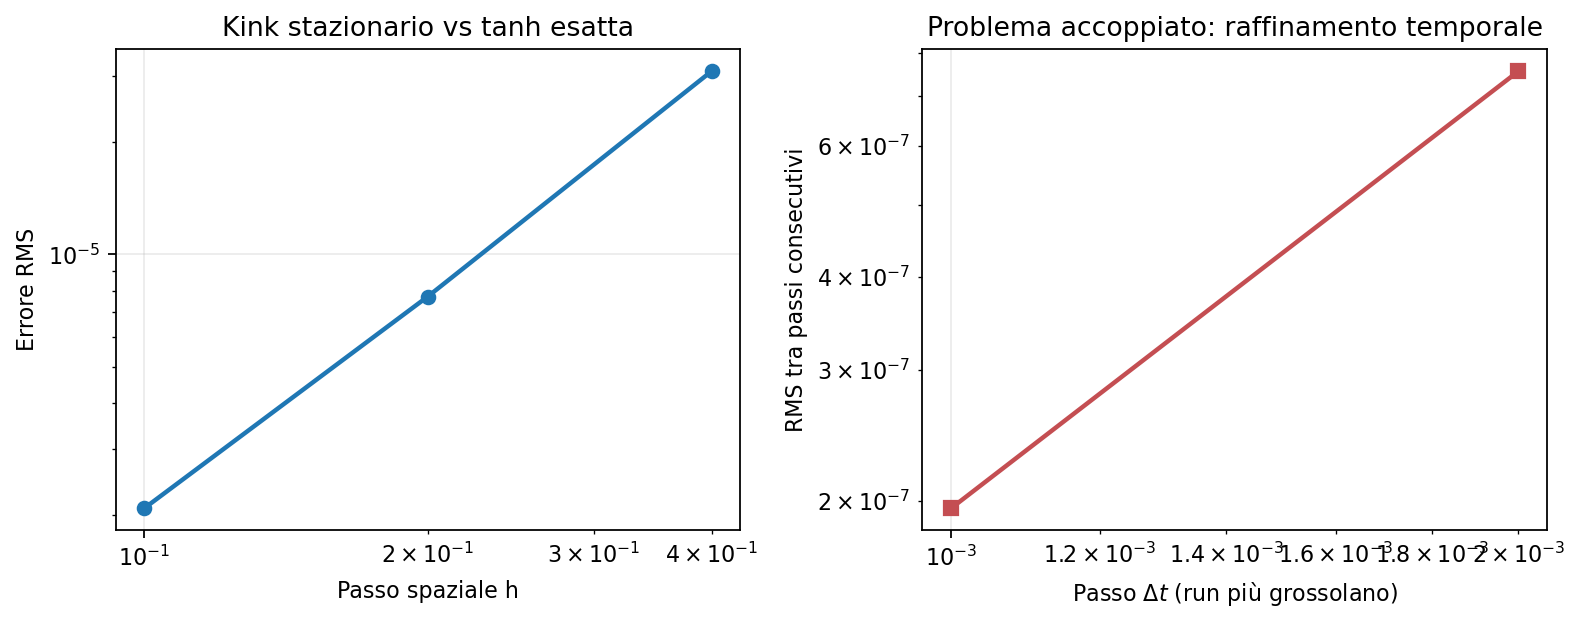
\includegraphics[width=.95\textwidth]{comparison_report_figures/hyperbolic_refinements.png}
\caption{A sinistra: convergenza spaziale del kink contro il profilo esatto. A destra: differenza tra passi temporali successivi per il caso accoppiato; il riferimento è la soluzione più fine, non una soluzione esatta.}
\end{figure}

\subsection{Onda viaggiante esatta di Nizovtseva et al.}
Nizovtseva, Galenko e Alexandrov studiano
\[
\tau\phi_{t't'}+\phi_{t'}=\Delta'\phi+\phi-\phi^3.
\]
Nel caso adimensionale $\tau=0.2$, la loro Eq.~(29) fornisce l'onda
\[
\phi(x',t')=\left[1+\exp\left(\frac{\sqrt{2+9\tau}}{2}x'-\frac32t'\right)\right]^{-1}.
\]
Abbiamo impostato $D=M=1$, $\rho=\tau=0.2$, coefficiente di reazione e mobilità unitari; il coefficiente di smorzamento fisico $1$ è implementato come \texttt{wavedamping=5}. La velocità iniziale nodale è quella esatta, $\phi_{t'}(x',0)=\frac32\phi(x',0)[1-\phi(x',0)]$. Il dominio computazionale $[-12,12]\times[0,1]$ usa condizioni naturali di Neumann sui bordi: la discrepanza con la coda esatta ai lati è esponenzialmente piccola. Si confrontano i campi al tempo $t'=0.2$ con la formula chiusa, senza dati digitalizzati e senza costruire una sorgente MMS.

Con $h=0.30,0.15,0.075$, gli errori RMS nodali sono $2.918\cdot10^{-5}$, $7.323\cdot10^{-6}$ e $1.862\cdot10^{-6}$; gli ordini osservati sono 1.995 e 1.976. La traiettoria è quindi riprodotta quantitativamente nel bulk e la convergenza è compatibile con elementi Q1. Il controllo temporale a $h=0.15$ è invece limitato dal plateau dell'errore spaziale: non lo usiamo per stimare in modo affidabile l'ordine temporale.
\begin{figure}[h!]
\centering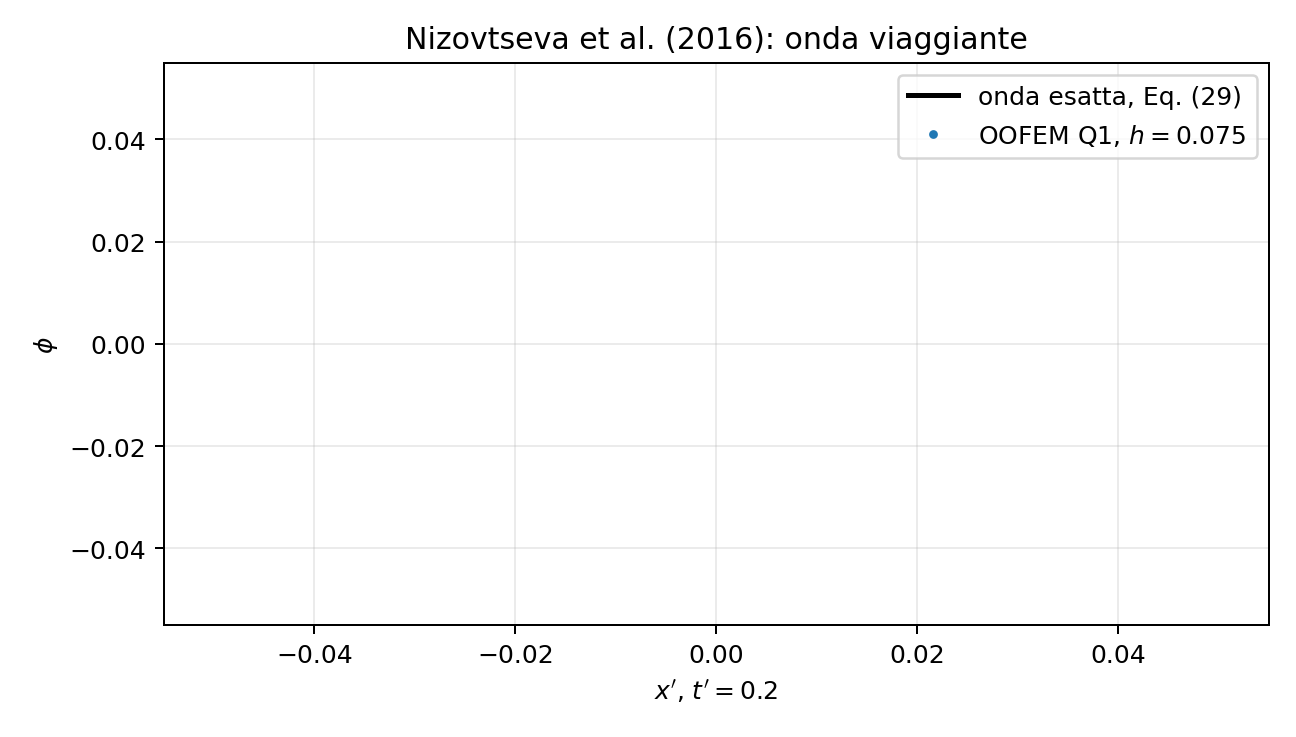
\includegraphics[width=.78\textwidth]{comparison_report_figures/nizovtseva_traveling_wave.png}
\caption{Onda viaggiante di Nizovtseva et al. a $t'=0.2$: profilo OOFEM e soluzione chiusa.}
\end{figure}
\begin{figure}[h!]
\centering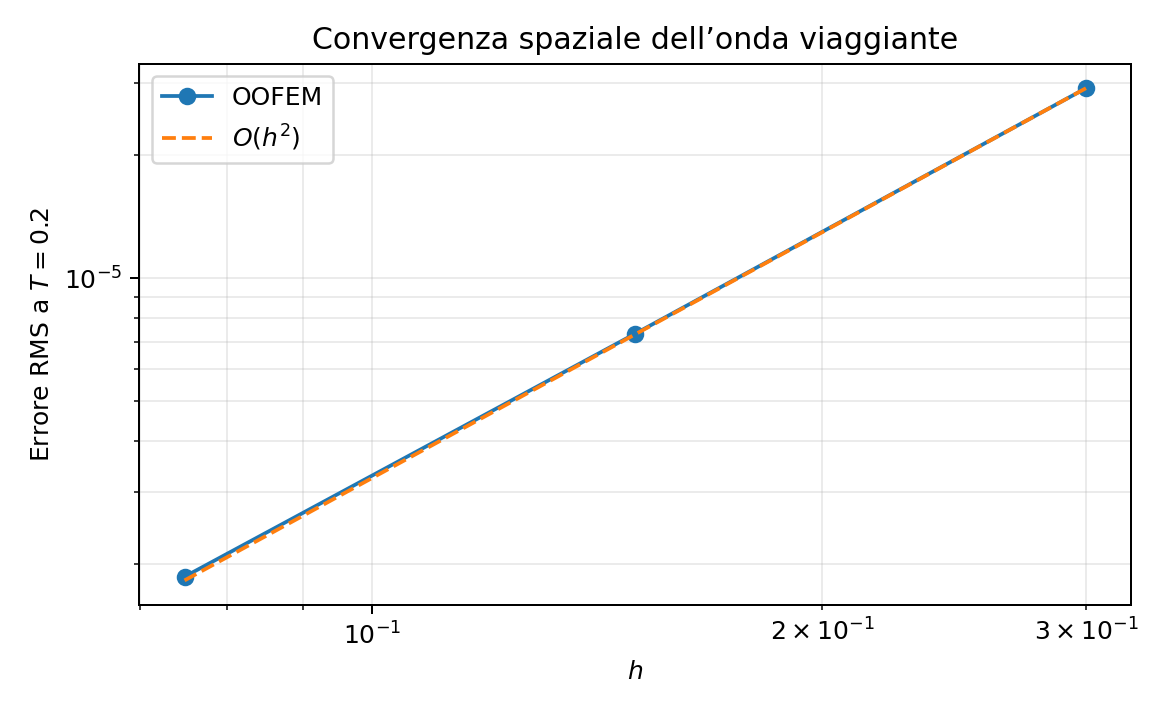
\includegraphics[width=.68\textwidth]{comparison_report_figures/nizovtseva_convergence.png}
\caption{Errore rispetto alla formula esatta al raffinarsi di $h$; la pendenza è circa due.}
\end{figure}

\subsection{Profilo esatto di Hochbruck--Leibold: verifica adattata, non replica diretta}
La versione corretta dell'articolo di Hochbruck e Leibold (e la relativa correzione) considera un'onda semilineare con inerzia nel bulk e sulla superficie, smorzamento/advezione nel bulk e un'equazione acustica sulla frontiera. Nel caso su disco unitario la soluzione esatta è $u(t,x)=\sin(2\pi t)x_1x_2$, con dati iniziali $u(0)=0$ e $u_t(0)=2\pi x_1x_2$. La forzante dell'articolo è costruita perché questo profilo soddisfi quel sistema.

Abbiamo usato la stessa geometria e lo stesso profilo/dato iniziale, ma ricalcolato il residuo per l'operatore effettivamente implementato da OOFEM: inerzia e smorzamento nel bulk, Allen--Cahn del primo ordine sulla superficie. Questa prova verifica il percorso input/output con un riferimento analitico indipendente sul profilo. Non è il benchmark numerico del paper: OOFEM non ha l'inerzia di superficie né i termini di trasporto/smorzamento spaziale bulk del modello di Hochbruck--Leibold, e la sorgente non coincide con quella pubblicata.

Sul disco approssimato da triangoli lineari, a $T=0.2$ la mesh di 502 nodi dà errore RMS $1.424\cdot10^{-2}$ e massimo $4.884\cdot10^{-2}$. Raffinando da 60 a 179 e 502 nodi, l'RMS passa da $2.121\cdot10^{-2}$ a $1.687\cdot10^{-2}$ e $1.424\cdot10^{-2}$: il tasso è basso e l'errore massimo quasi non cala. I risultati temporali a 179 nodi sono invece stabili al diminuire di $\Delta t$ (RMS $1.689\cdot10^{-2}$, $1.687\cdot10^{-2}$, $1.687\cdot10^{-2}$), segno che qui domina l'errore spaziale/geometrico. I vertici del bordo poligonale e la rappresentazione lineare del disco limitano questa approssimazione; non dichiariamo convergenza spaziale soddisfacente né validazione del riferimento. Per una replica diretta servirebbe prima implementare nel solver l'equazione acustica accoppiata al bordo, poi usare il caso del paper senza alterarne il residuo.
\begin{figure}[h!]
\centering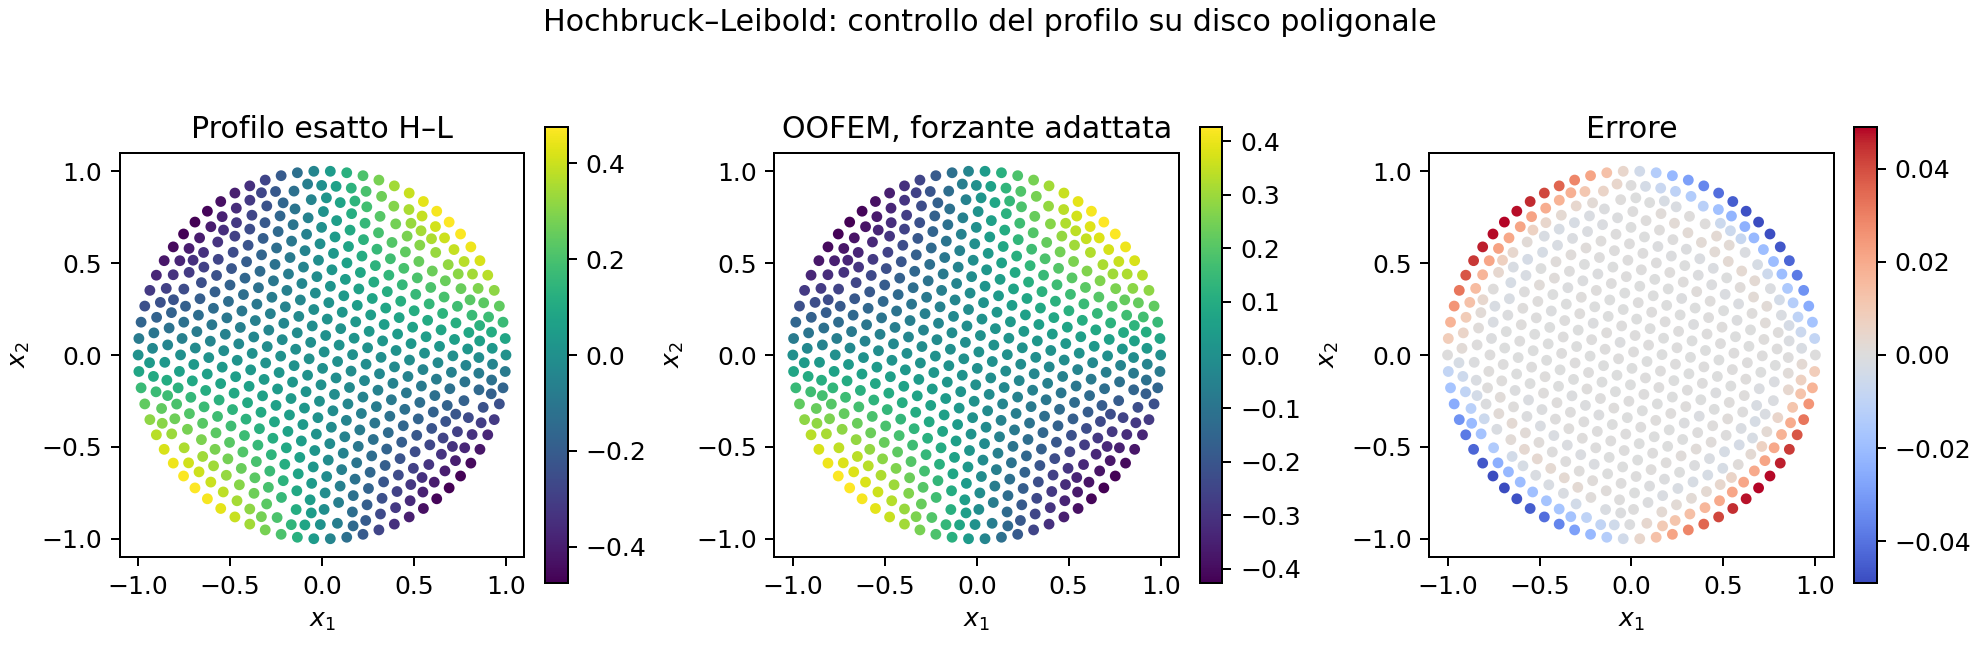
\includegraphics[width=.95\textwidth]{comparison_report_figures/hochbruck_leibold_adapted_profile.png}
\caption{Profilo esatto e campo numerico per la prova adattata alla legge OOFEM; il pannello errore mostra la discrepanza spaziale residua.}
\end{figure}

\subsection{Confronto con la teoria di Calatroni--Colli}
Qui il confronto teorico è possibile, ma va formulato correttamente: Calatroni--Colli non forniscono una formula chiusa $u(x,t)$ per questi dati. I Teoremi 2.3--2.5 dimostrano dipendenza continua dai dati, unicità e, sotto ipotesi aggiuntive, esistenza di una soluzione debole. Questa soluzione unica è il limite teorico a cui deve approssimare la discretizzazione quando si raffinano spazio e tempo.

Per il doppio pozzo polinomiale usato da OOFEM si può porre $\beta(r)=\beta_\Gamma(r)=r^3$, con primitiva convessa $\widehat\beta(r)=r^4/4$, e $\pi(r)=\pi_\Gamma(r)=-r$. Si recuperano così $u^3-u$ nel bulk e sulla frontiera; la scelta soddisfa la compatibilità tra le non linearità bulk e superficiale richiesta dal teorema. Nel test 2D con $c=k=\texttt{mobility}=\texttt{surfacebeta}=1$, senza forzanti e con dato iniziale liscio, anche la forma delle equazioni corrisponde al modello teorico. La mesh è un quadrato poligonale, mentre il testo assume un dominio regolare: questa è la riserva geometrica del confronto.

Abbiamo quindi confrontato la soluzione numerica con le conseguenze verificabili della teoria, non con valori puntuali inesistenti: riducendo $\Delta t$ da $0.005$ a $0.0025$ e poi a $0.00125$, la differenza RMS nodale tra i campi finali successivi si dimezza quasi esattamente ($2.285\cdot10^{-4}$ e $1.159\cdot10^{-4}$), coerentemente con backward Euler di primo ordine. Raffinando la mesh da $10\times10$ a $20\times20$, l'RMS nodale rispetto alla mesh $40\times40$ scende da $1.279\cdot10^{-4}$ a $2.590\cdot10^{-5}$. La soluzione più fine è un riferimento numerico, non la soluzione teorica esatta. Questi risultati sono evidenza di convergenza verso la soluzione debole unica, ma non costituiscono da soli una dimostrazione di convergenza dello schema.
\begin{figure}[h!]
\centering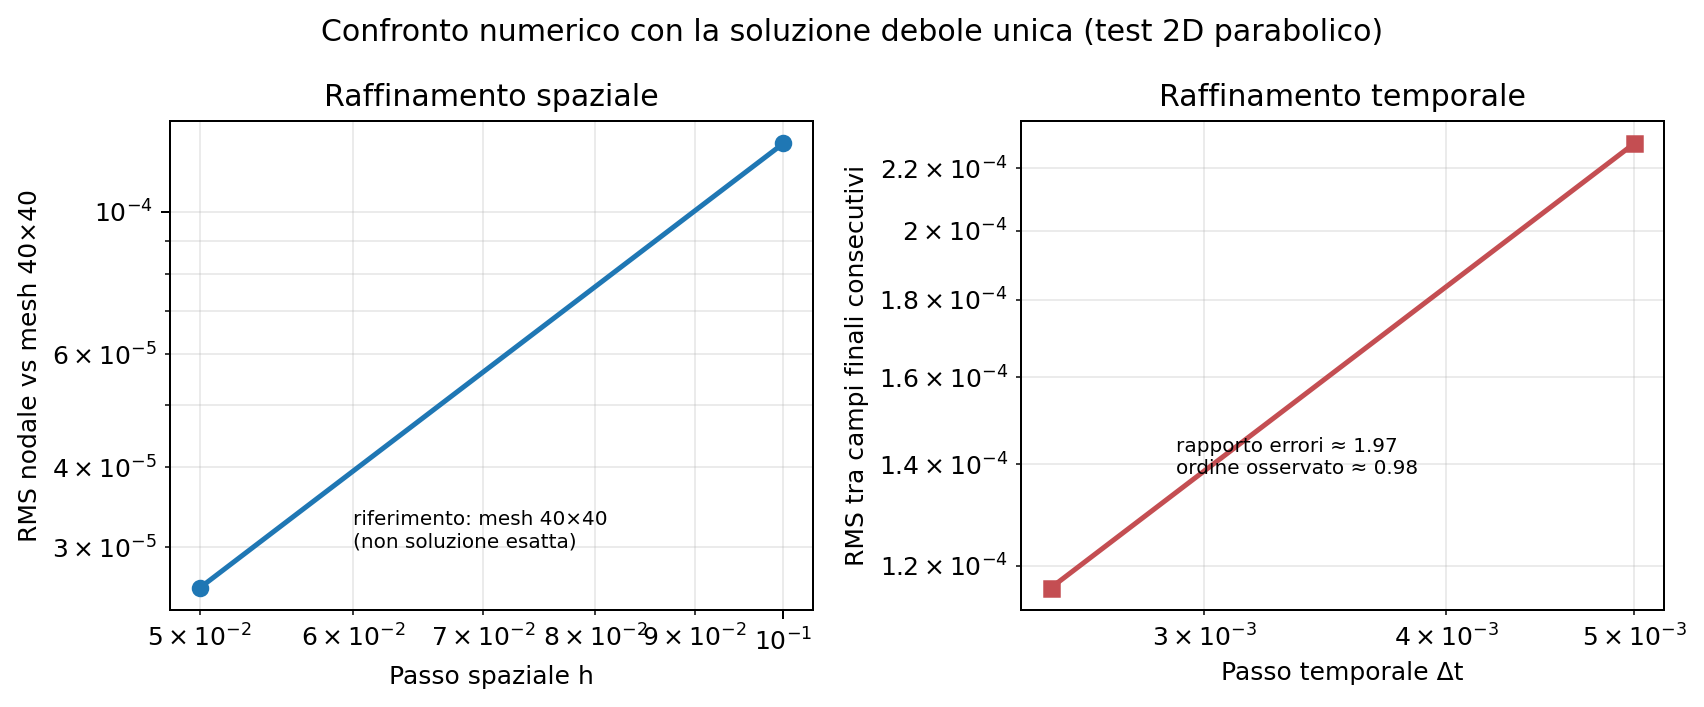
\includegraphics[width=.92\textwidth]{comparison_report_figures/calatroni_colli_refinement.png}
\caption{Raffinamenti del test parabolico 2D che realizza il modello polinomiale di Calatroni--Colli. I riferimenti sono campi OOFEM più fini; il teorema garantisce unicità del limite continuo, ma non dà una soluzione chiusa da sovrapporre.}
\end{figure}

\subsection{Che cosa aggiungono le altre nuove fonti}
La versione riveduta di Hipp--Kovács (CRC 2018/53, 2020) contiene benchmark FEM 2D con inerzia dinamica al bordo, quindi non direttamente sovrapponibili. La prova adattata di Hochbruck--Leibold descritta sopra sfrutta invece la loro soluzione esatta come profilo di riferimento, mantenendo esplicito il cambio di equazione.

\subsection*{Verdetto iperbolico}
La replica di Nizovtseva è un confronto diretto favorevole per l'equazione iperbolica bulk: onda viaggiante esatta e ordine spaziale circa due. Il profilo esatto di Hochbruck--Leibold è stato confrontato numericamente solo dopo aver adattato la forzante al modello OOFEM; il risultato è esplorativo e mostra errore spaziale ancora significativo. Rimane da validare l'accoppiamento bulk-superficie contro un benchmark pubblicato con la stessa legge dinamica al bordo.

\section{Conclusioni operative}
\begin{center}\begin{tabular}{p{.20\textwidth}p{.29\textwidth}p{.39\textwidth}}
\toprule
Ramo & Stato sostenuto dai dati & Limite principale \\
\midrule
Parabolico 1D & Confronto quantitativo favorevole con energia di Okumura & Curva digitalizzata da figura; geometria 1D estrusa in OOFEM \\
Parabolico 2D & Raffinamenti coerenti con unicità teorica di Calatroni--Colli; test Xiao--Chen qualitativo & Riferimento numerico spaziale, non soluzione esatta; nel caso Xiao--Chen $\varepsilon$ non dichiarato \\
Iperbolico bulk & Onda viaggiante di Nizovtseva: accordo con formula esatta, ordine spaziale $\approx2$ & Benchmark bulk, condizioni Neumann su dominio troncato \\
Profilo H--L adattato & Controllo analitico eseguito, ma RMS $1.42\cdot10^{-2}$ e raffinamento spaziale debole & Non replica l'equazione H--L; frontiera OOFEM diversa \\
\bottomrule
\end{tabular}\end{center}

La formulazione prudente è dunque: il ramo parabolico ha un confronto quantitativo di letteratura nel caso 1D e un confronto con le conseguenze teoriche di Calatroni--Colli nel caso 2D. Nel ramo iperbolico il bulk è confrontato direttamente con l'onda esatta di Nizovtseva; il caso Hochbruck--Leibold è soltanto una verifica di profilo adattata, non una replica del loro benchmark. Il modello accoppiato di OOFEM resta da validare contro una soluzione di letteratura con la stessa equazione al bordo.

\section*{Riferimenti}
{\small\begin{enumerate}\setlength{\itemsep}{0pt}
\item M. Okumura, \emph{Design and analysis of structure-preserving schemes for parabolic partial differential equations with dynamic boundary conditions}, tesi di dottorato, Osaka University (2021), cap. 4, es. 2. \href{https://doi.org/10.18910/82279}{DOI}
\item M. Xiao, R. Chen, \emph{A first-order energy stable scheme for the Allen--Cahn equation with the Allen--Cahn type dynamic boundary condition}, J. Comput. Appl. Math. 460 (2025), 116409. \href{https://doi.org/10.1016/j.cam.2024.116409}{DOI}
\item I. G. Nizovtseva, P. K. Galenko, D. V. Alexandrov, \emph{The hyperbolic Allen--Cahn equation: exact solutions}, J. Phys. A 49 (2016), 435201. \href{https://doi.org/10.1088/1751-8113/49/43/435201}{DOI}
\item L. Calatroni, P. Colli, \emph{Global solution to the Allen--Cahn equation with singular potentials and dynamic boundary conditions}, arXiv:1206.6738 (2012).
\item D. Hipp, B. Kovács, \emph{Finite element error analysis of wave equations with dynamic boundary conditions: $L^2$ estimates}, CRC 1173 Preprint 2018/53, revised 2020.
\item M. Hochbruck, T. Leibold, \emph{Finite element discretization of semilinear acoustic wave equations with kinetic boundary conditions}, CRC 1173 Preprint 2019/26.
\item M. Hochbruck, T. Leibold, \emph{An implicit-explicit time discretization scheme for second-order semilinear wave equations with application to dynamic boundary conditions}, Numer. Math. 147 (2021), 869--899, DOI: \href{https://doi.org/10.1007/s00211-021-01184-w}{DOI}; correzione: DOI \href{https://doi.org/10.1007/s00211-021-01190-y}{DOI}.
\end{enumerate}}
\vfill\noindent\small Input, script, metriche CSV e figure delle prove iperboliche sono nella cartella \url{doc/stvowu_validation/hyperbolic/}; istruzioni e limiti sono nel relativo README.
\end{document}
